\documentclass[onecolumn, 11pt, letterpaper]{article}

\usepackage{listings}
\lstset{language=C}

\usepackage{cmu-techreport}
%\usepackage{comment}
\newcommand{\graphtype}{monochrome}

% PDF 
\usepackage[%
  draft=false,
  colorlinks=true,     % color the words instead of use a colored box
  urlcolor=blue,       % \href{...}{...} external (URL)
  filecolor=blue,      % \href{...} local file
  linkcolor=black,     % \ref{...} and \pageref{...}
  citecolor=black,     % \cite{}
%  pdftitle={},
%  pdfauthor={},
%  pdfsubject={},
%  pdfkeywords={},
%  pdfproducer={pdfLaTeX},
%  pagebackref,        % backward references in the bibliography
  pdfpagemode=UseOutlines,  % None, UseThumbs, UseOutlines, FullScreen
  bookmarksopen=true   % Does outline start expanded?
  ]{hyperref}

\topmargin      -0.3in
\headheight     0in
\headsep        0.3in
\textheight     9.0in
\oddsidemargin  0pt
\evensidemargin \oddsidemargin
\marginparwidth 0.5in
\textwidth      6.5in
\renewcommand{\baselinestretch}{1.0}
\renewcommand{\baselinestretch}{1.0}
%\parindent 0.3in
\parindent -0.6in

% Math
\usepackage[fleqn]{amsmath}
\usepackage{amssymb}
\usepackage{amsthm}
\usepackage[mathscr]{eucal} % \mathcal and \mathscr for fancy calligraphy.
 
% Fonts
%\usepackage{mathptmx} % Times for body and for math symbols
%\usepackage{helvet}   % Helvetica for \mathsf
%\usepackage{courier}  % Courier for \mathtt


% Everything else
\usepackage[table]{xcolor}
\usepackage{color}
\usepackage{colortbl}
\usepackage[pdftex,final]{graphicx}
							 % actually include eps files when you build.
\usepackage{url}
\usepackage{hhline}        % fancy table lines
\usepackage{tabularx}      % tables that auto-size
% \usepackage[font={small},labelfont={bf},labelsep=period,margin=10pt,aboveskip=6pt,belowskip=-5pt]{caption}
\usepackage[labelfont={bf},labelsep=period,margin=10pt]{caption}
% Can do ``belowskip=-5pt'' to tighten up spacing further...
% Or, can change \setlength\dbltextfloatsep{10pt plus 2pt} in usetex class file.
%\usepackage{algorithmic}
%\usepackage{verbatim}
\usepackage[figuresright]{rotating}

%%%%%% Tables and figures
%%%%%%
\usepackage[pdftex]{graphicx}           %%%%% PDFLATEX (for PDF figures)
\usepackage{lscape}                     %%%%% Landscape rotation
\usepackage{rotating}                   %%%%% ?
\usepackage{booktabs}                   %%%%% ?
\usepackage[table]{xcolor}              %%%%% Colors in tables

%%%%%% Misc
%%%%%%
\usepackage{verbatim}                   %%%%% Block comments (\begin{comment}) 
\usepackage{color}                      %%%%% Graphics
\usepackage{thumbpdf}                   %%%%% ?
\usepackage{url}                        %%%%% URL formatting

\pagestyle{plain} % has page numbers

\begin{document}

% Compact itemize and enumerate.  Note that they use the same counters and
% symbols as the usual itemize and enumerate environments.
\def\compactify{\itemsep=0pt \topsep=0pt \partopsep=0pt \parsep=0pt}
\let\latexusecounter=\usecounter
\newenvironment{CompactItemize}
  {\def\usecounter{\compactify\latexusecounter}
   \begin{itemize}}
  {\end{itemize}\let\usecounter=\latexusecounter}
\newenvironment{CompactEnumerate}
  {\def\usecounter{\compactify\latexusecounter}
   \begin{enumerate}}
  {\end{enumerate}\let\usecounter=\latexusecounter}

\newcommand{\bci}{\begin{CompactItemize}\addtolength{\itemsep}{-0.075in}}
\newcommand{\eci}{\end{CompactItemize}}
\newcommand{\bce}{\begin{CompactEnumerate}}
\newcommand{\ece}{\end{CompactEnumerate}}

%-- place any standard commands/environments here to get included in
%-- documents.  When you include this file, you should do it before
%-- the \begin{document} tag.

%%%%%%%%%%%%%%%%%%%%%%%%%%%%%%%%%%%%%%%%%%%%%%%%%%%%%%%%%%%%%%%%
% Special font and spacing formatting

%-- Terms...  Use this to introduce a term in the paper.
\newcommand{\term}[1]{\emph{#1}}

%-- Provides fixed width font for code snippets.
% \newcommand{\code}[1]{\texttt{\textbf{#1}}}
% \newcommand{\code}[1]{\textsc{\texttt{#1}}}
\newcommand{\code}[1]{\texttt{#1}}

%-- Commands: e.g., WRITE command.
\newcommand{\command}[1]{{\textsc \MakeLowercase{#1}}}

%-- Jiri caption
\newcommand{\minicaption}[2]{\caption[#1]{\textbf{#1.} #2}}

% Unit(s)
%-- unit: 4KB -> 4\unit{KB}
\newcommand{\unit}[1]{\,#1} % thin space followed by units
%-- Units on numbers: 4KB -> \units{4}{KB}
\newcommand{\units}[2]{#1\unit{#2}}
% Specific units...
\newcommand{\micros}{\ensuremath{\mu}{s}}

%-- Inline title
\newcommand{\inlinesection}[1]{\smallskip\noindent{\textbf{#1.}}}

%%%%%%%%%%%%%%%%%%%%%%%%%%%%%%%%%%%%%%%%%%%%%%%%%%%%%%%%%%%%%%%%
% Editting commands

%-- For notes about things that need to be fixed.
\newcommand{\fix}[1]{~{\LARGE\ensuremath{\star}}~\textbf{#1}~{\LARGE\ensuremath{\star}}~}

\newcommand{\bcut}{\marginpar{\ensuremath{\bigvee}}}
\newcommand{\ecut}{\marginpar{\ensuremath{\bigwedge}}}

%-- Draft watermark in upperleft corner
\newcommand{\reviewtimetoday}[2]{\special{!userdict begin
/bop-hook{gsave 20 710 translate 45 rotate 0.8 setgray
/Times-Roman findfont 12 scalefont setfont 0 0   moveto (#1) show
0 -12 moveto (#2) show grestore}def end}}


%%%%%%%%%%%%%%%%%%%%%%%%%%%%%%%%%%%%%%%%%%%%%%%%%%%%%%%%%%%%%%%%
% Table and Figure formatting

% Table format
% inter-row spacing for tables
\renewcommand{\arraystretch}{1.0}
% Control spacing of ``double lines'' (default is 2pt)
% Can set this within braces but before \begin{table}...
%\setlength{\doublerulesep}{0.2mm} % into a single think line
% \setlength{\doublerulesep}{3pt} % obvious spacing.
\setlength{\tabcolsep}{1pt} % default is 6pt

% Table commands
% font size for tables
%\newcommand{\tablefontsize}{\scriptsize}
%\newcommand{\tablefontsize}{\footnotesize}
\newcommand{\tablefontsize}{\small}
%\newcommand{\tablefontsize}{}

% \usepackage{tabularx}
% Using L, C, R as the column type will left, center, or right justify text.
\newcolumntype{L}{X}
\newcolumntype{C}{>{\centering\arraybackslash}X}
\newcolumntype{R}{>{\raggedleft\arraybackslash}X}

% Figure commands
\newcommand{\figurewidth}{\columnwidth}

% algorithm / pseudo-code
\newcommand{\pseudosize}{\scriptsize}
\newcommand{\pseudowidth}{\columnwidth}
\newcommand{\pseudoskip}{\smallskip}
%\newcommand{\pseudoskip}{}

% pseudo-code commands
\newcommand{\ccomment}[1]{ /$*$ #1 $*$/}	
\newcommand{\rccomment}[1]{\hfill\ccomment{#1}} % right aligns the comment

%%%%%%%%%%%%%%%%%%%%%%%%%%%%%%%%%%%%%%%%%%%%%%%%%%%%%%%%%%%%%%%%
% Math. Uses package ``amsthm''.

%-- Influenced by the ACM journal tex template
%\newtheorem{theorem}{Theorem}[section]
%\newtheorem{conjecture}[theorem]{Conjecture}
%\newtheorem{corollary}[theorem]{Corollary}
%\newtheorem{proposition}[theorem]{Proposition}
%\newtheorem{lemma}[theorem]{Lemma}
%\theoremstyle{definition} % This currently does nothing...
%\newtheorem{definition}[theorem]{Definition}
%\newtheorem{observation}[theorem]{Observation}
%\newtheorem{remark}[theorem]{Remark}

%%-- Referencing Lemma, Observation, Definition
%\newcommand{\thmref}[1]{Theorem~\ref{#1}}
%\newcommand{\lemref}[1]{Lemma~\ref{#1}}
%\newcommand{\defref}[1]{Definition~\ref{#1}}

%%-- Examine different math fonts 
%%-- \usepackage{amsmath}
%%-- \usepackage[mathscr]{eucal} % \mathcal and \mathscr for fancy calligraphy.
%\newcommand{\mathfonts}[1]{ \text{math:~} {#1},\\ \text{mathsf:~} \mathsf{#1},\\ \text{mathcal:~} \mathcal{#1}\\ \text{mathscr:~} \mathscr{#1},\\ \text{mathrm:~} \mathrm{#1},\\ \text{mathbb:~} \mathbb{#1},\\ \text{mathbf:~} \mathbf{#1},\\ \text{mathtt:~} \mathtt{#1}}


%%%%%%%%%%%%%%%%%%%%%%%%%%%%%%%%%%%%%%%%%%%%%%%%%%%%%%%%%%%%%%%%
% Lists
\newenvironment{outline}
{
	\renewcommand{\baselinestretch}{1.0}
	\footnotesize
    \begin{list}
    {--} % Leave empty for nothing, or replace bullet with any other symbol.
    {
        \setlength{\partopsep}{0in}
        \setlength{\topsep}{0in}
        \setlength{\parsep}{0in}
        \setlength{\itemsep}{0in}
        \setlength{\leftmargin}{0.3in}
    }
}
{
    \end{list}
}


% Lists with single spacing
\newenvironment{my_enumerate}{
\begin{enumerate}
  \setlength{\partopsep}{0in}
  \setlength{\topsep}{0in}
  \setlength{\itemsep}{1pt}
  \setlength{\parskip}{0pt}
  \setlength{\parsep}{0pt}
}{\end{enumerate}}

\newenvironment{my_description}{
\begin{description}
  \setlength{\partopsep}{0in}
  \setlength{\topsep}{0in}
  \setlength{\itemsep}{1pt}
  \setlength{\parskip}{0pt}
  \setlength{\parsep}{0pt}
}{\end{description}}

\newenvironment{my_itemize}{
\begin{itemize}
  \setlength{\partopsep}{0in}
  \setlength{\topsep}{0in}
  \setlength{\itemsep}{1pt}
  \setlength{\parskip}{0pt}
  \setlength{\parsep}{0pt}
}{\end{itemize}}

\newenvironment{my_list}{
\begin{list}{}{
%  \setlength{\itemindent}{\leftmargin}
  \setlength{\topsep}{0in}
  \setlength{\partopsep}{0in}
  \setlength{\topsep}{0in}
  \setlength{\itemsep}{1pt}
  \setlength{\parskip}{0pt}
  \setlength{\parsep}{0pt}
}}{\end{list}}



\hyphenation{OpenAFS}
\hyphenation{FSVA}


\newcommand{\sys}{\textsc{SkyeFS}}      %%%%%% SYSTEM NAME
\newcommand{\AUTHORS}{\textsc{Anthony Chivetta, Swapnil Patil \& Garth Gibson}}
\newcommand{\CONTACT}{\textit{Carnegie Mellon University}}
\newcommand{\EMAIL}{\texttt{anthony @ chivetta.org, \{swapnil.patil , garth.gibson\} @ cs.cmu.edu}}
\newcommand{\TITLE}{\textbf{SkyeFS:} \\ 
\textbf{Distributed Directories using Giga+ and PVFS}%~\thanks{~\NOTICE}
}

\title{
\textbf{SkyeFS:}\\
\textbf{Distributed Directories using Giga+ and PVFS}
}
\author{\AUTHORS \\~\\ \EMAIL}

\date{May 2012}
\trnumber{CMU-PDL-12-XXX}

\abstract{
  \small
  \it{
  There is growing set of large-scale data-intensive applications that require
  file system directories to store millions to billions of files in each
  directory and to sustain hundreds of thousands of concurrent directory
  operations per second. Unfortunately most cluster file systems are unable to
  provide this level of scale and parallelism.  In this research, we show how
  the GIGA+ distributed directory algorithm, developed at CMU, can be applied
  to a real-world cluster file system.  We designed and implemented a
  user-level file system, called SkyeFS, that efficiently layers GIGA+ on top
  of the PVFS cluster file system.  Our experimental evaluation demonstrates
  how an optimized interposition layer can help PVFS achieve the desired
  scalability for massive file system directories.
  }
}

\maketitle

\parindent 0.3in

\section{Overview}
PVFS, the Parallel Virtual File System, stores all metadata for a particular
directory on a single metadata server\cite{pvfs} resulting in poor scalability in the case
of large or high traffic directories.  Giga+ is a scheme for partitioning the
metadata for a directory across a set of servers while still maintaining
performance for small directories.\cite{gigaplus}  SkyeFS implements the Giga+ algorithms on
top of an unmodified PVFS file system.

SkyeFS consists of a client (\code{skye\_\-client}) which functions as the
FUSE filesystem and a server (\code{skye\_\-server}) which provides
synchronization for metadata operations and controls directory placement and
splitting.\cite{fuse}  

Giga+ incrementally splits a directory into multiple partitions which are
load-balanced across available servers.  In SkyeFS, we represent each
partition as a distinct PVFS directory.  A SkyeFS server located with each
PVFS metadata server (MDS) provides the synchronization and coordination for
the partitions on the local PVFS MDS. 

\section{Implementation Overview}
We choose to implement Giga+ as an overlay filesystem on top of PVFS, instead
of modifying PVFS directly, in hopes of keeping the implementation small and
simple.  FUSE provides an obvious choice for implementing the client side of
the system due to the ease of writing a FUSE file system driver.
Additionally, the pvfs2\-fuse application distributed with the PVFS source
provides an example of how to implement FUSE operations in PVFS.  However,
unlike pvs2\-fuse, we use the lowlevel FUSE API.  This allows us to directly
specify the inode numbers returned to the kernel, avoiding extraneous pathname
resolution in the client by using PVFS handles as inode numbers.

In PVFS, every object is assigned a PVFS metadata handle and each PVFS server
is statically assigned a range of handles for which it is responsible.  
The directory entries in a directory are stored with that directory's metadata
on the server responsible for its metadata handle.  We exploit this property
of PVFS to manipulate metadata placement for each Giga+ partition.

\subsection{Filesystem Layout}
SkyeFS establishes a direct mapping between Giga+ partitions and a set of PVFS
directories.  This allows us to use Giga+ to both achieve load-balancing and
keep overall directory size small.  Rename operations in PVFS are relatively
cheep as they only move object metadata and not entire files.  This helps limit
the cost of any extra renames required by this storage scheme.  In systems
where this is not the case, a single directory per metadata server might be
used instead.

When a logical directory is created, we also create a PVFS directory on the
same server called ``p00000'' inside the logical directory to represent the
first Giga+ partition.  When this partition splits, a new directory ``p00001''
will be created adjacent to it to store the files in the new partition.  

The PVFS client uses round-robin assignment for selecting the metadata server
on which it will create a new  object.  Unfortunately, the PVFS client API
does not currently provide any way to influence this server selection.  When
creating PVFS directories for new partitions, we work around the problem by
repeatedly creating new directories until the resulting directory is on the
correct server.  Future versions of SkyeFS might cache these directories to
limit extraneous creates.

\subsection{Client/Server Architecture}
\begin{figure}
\begin{center}
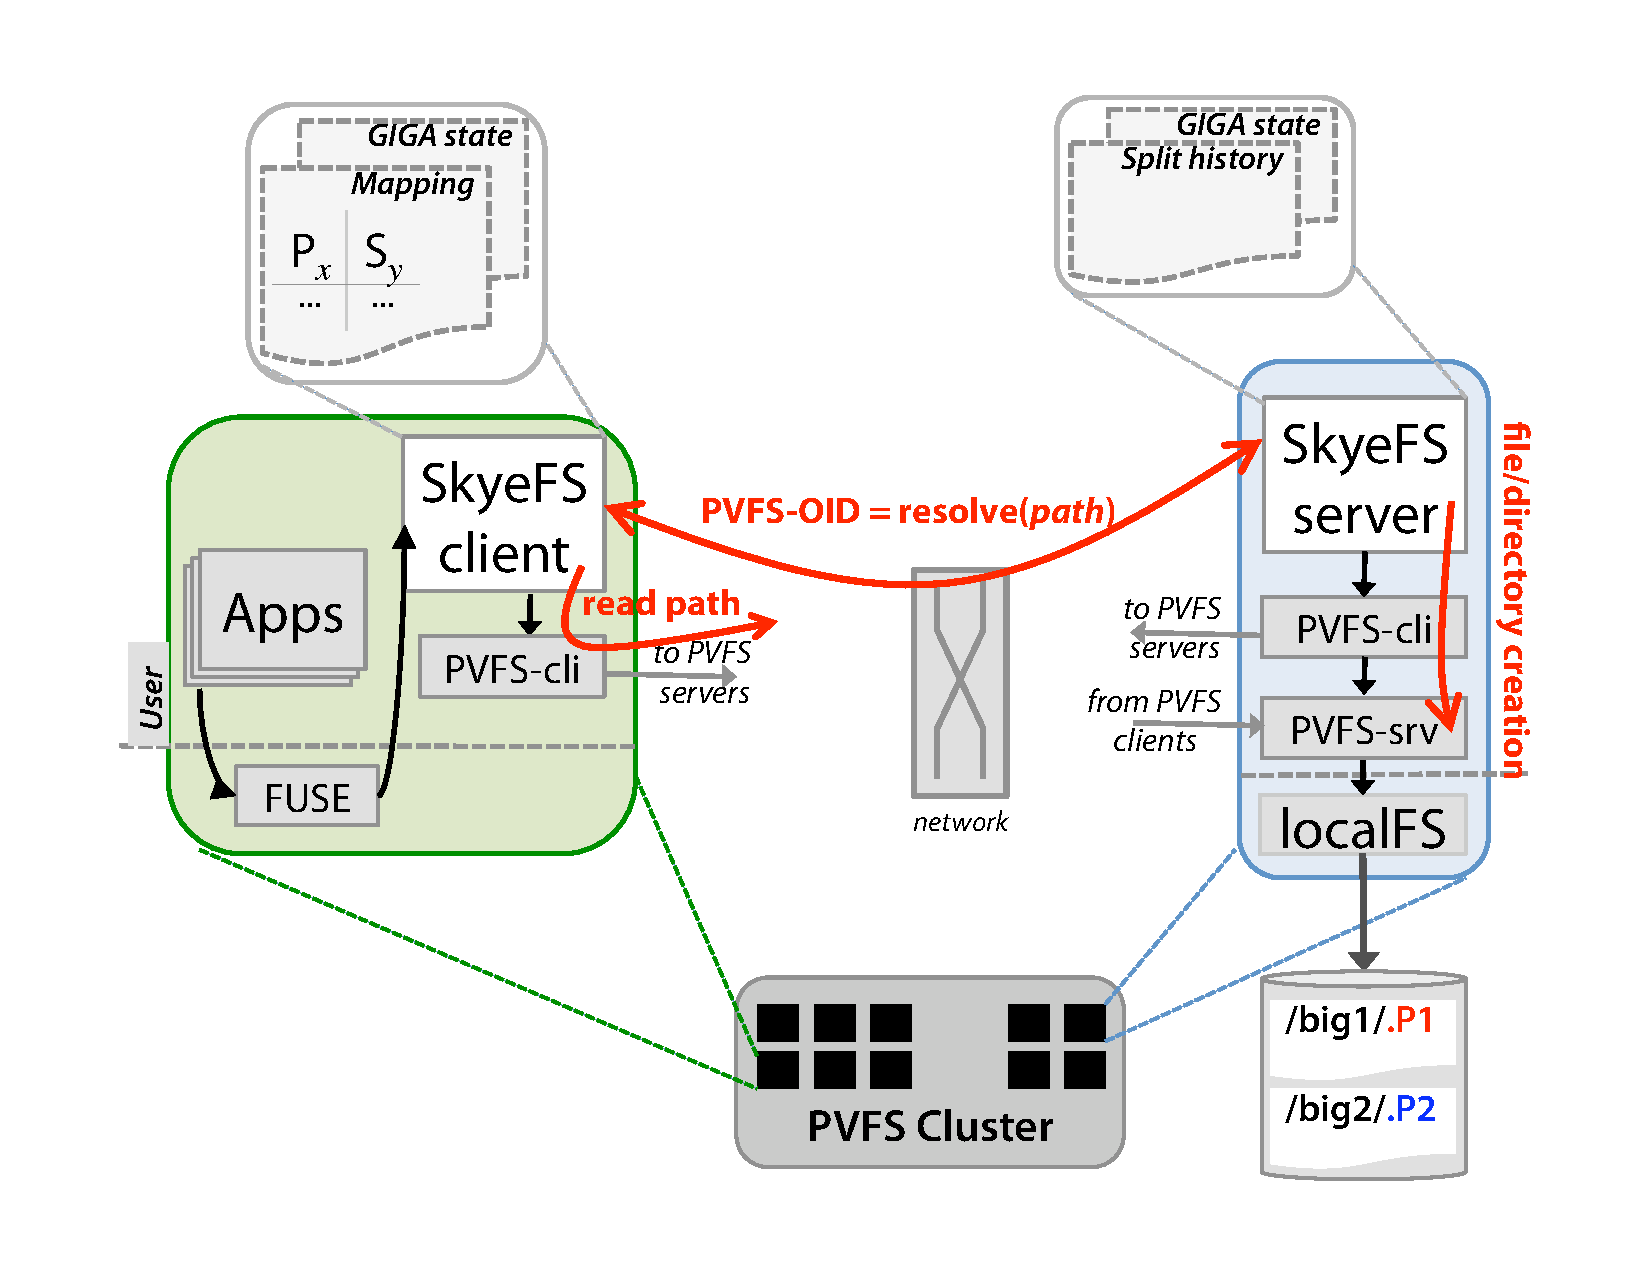
\includegraphics[width=3in]{figure-architecture}
\end{center}
\caption{SkyeFS Architecture Diagram}
\end{figure}

\begin{figure}
\begin{lstlisting}
struct skye_directory {
    giga_mapping mapping;
    int reference_count;
    PVFS_object_ref PVFS_handle;
    int splitting_index;
    pthread_rwlock_t rwlock;
    UT_hash_handle hashtable_handle;
};
\end{lstlisting}
\caption{Giga+ Directory Metadata}
\label{fig:skyedir}
\end{figure}

Giga+ has metadata that it must maintain in order to manage each directory's
partitions.  SkyeFS uses a small server process, \code{skye\_server}, located
on each PVFS server to manage this metadata and ensure consistency for the
directories and partitions resident on that server.  The \code{skye\_server}
has a cache of \code{skye\_directory} structures which store this metadata.
This metadata can be regenerated from PVFS at any time, allowing the
\code{skye\_server} to fail or evict items from its cache at any time without
the risk of leaving the system in an inconsistent state.

Each client runs a \code{skye\_client} process that provides a FUSE filesystem
and issues requests to the \code{skye\_server}s using ONC RPC and PVFS using
the PVFS system interface.\cite{rpc}  For most operations, the client is a simple
adaption of the \code{pvfs2-fuse} code to use the lowlevel FUSE API.  However,
metadata operations which require path name resolution or object creation are
forwarded through the \code{skye\_server} to prevent race conditions.  To
speed operation, the client also maintains a cache of the \code{giga\_mapping}
for recently accessed directories.

For performance and load-balance reasons, locality between the
\code{skye\_\-server} process and the PVFS server to which it is making
requests is maintained whenever possible.  Upon receiving a RPC request, the
server will first check if it owns the partition to be accessed by the
request.  If not, the server will return the error EAGAIN and provide
the client with a copy of its own mapping for the directory.  Upon receiving
this error, the client will read the server provided mapping and merge that
information with its local version.  The client will then reattempt the RPC
call to the new \code{skye\_\-server} as per the updated mapping.  This
ensures both that locality is maintained and that the client's cached mapping
will tend toward reality.

The most important job of the \code{skye\_server} is to prevent race
conditions during splitting.  Any operation that must resolve a pathname (such
as a lookup, create, or rename) needs to have an accurate Giga+ bitmap for the
directory so that they can operate on the correct partition.  By forwarding
these operations to the \code{skye\_server}, the server can ensure they happen
without interference from changing bitmaps.  There do exist schemes that would
allow client applications do so some of these operations without the server in
an optimistic manor; however, such schemes are error prone and overly
complicated.

\subsection{Path Resolution}
\begin{figure}
\begin{center}
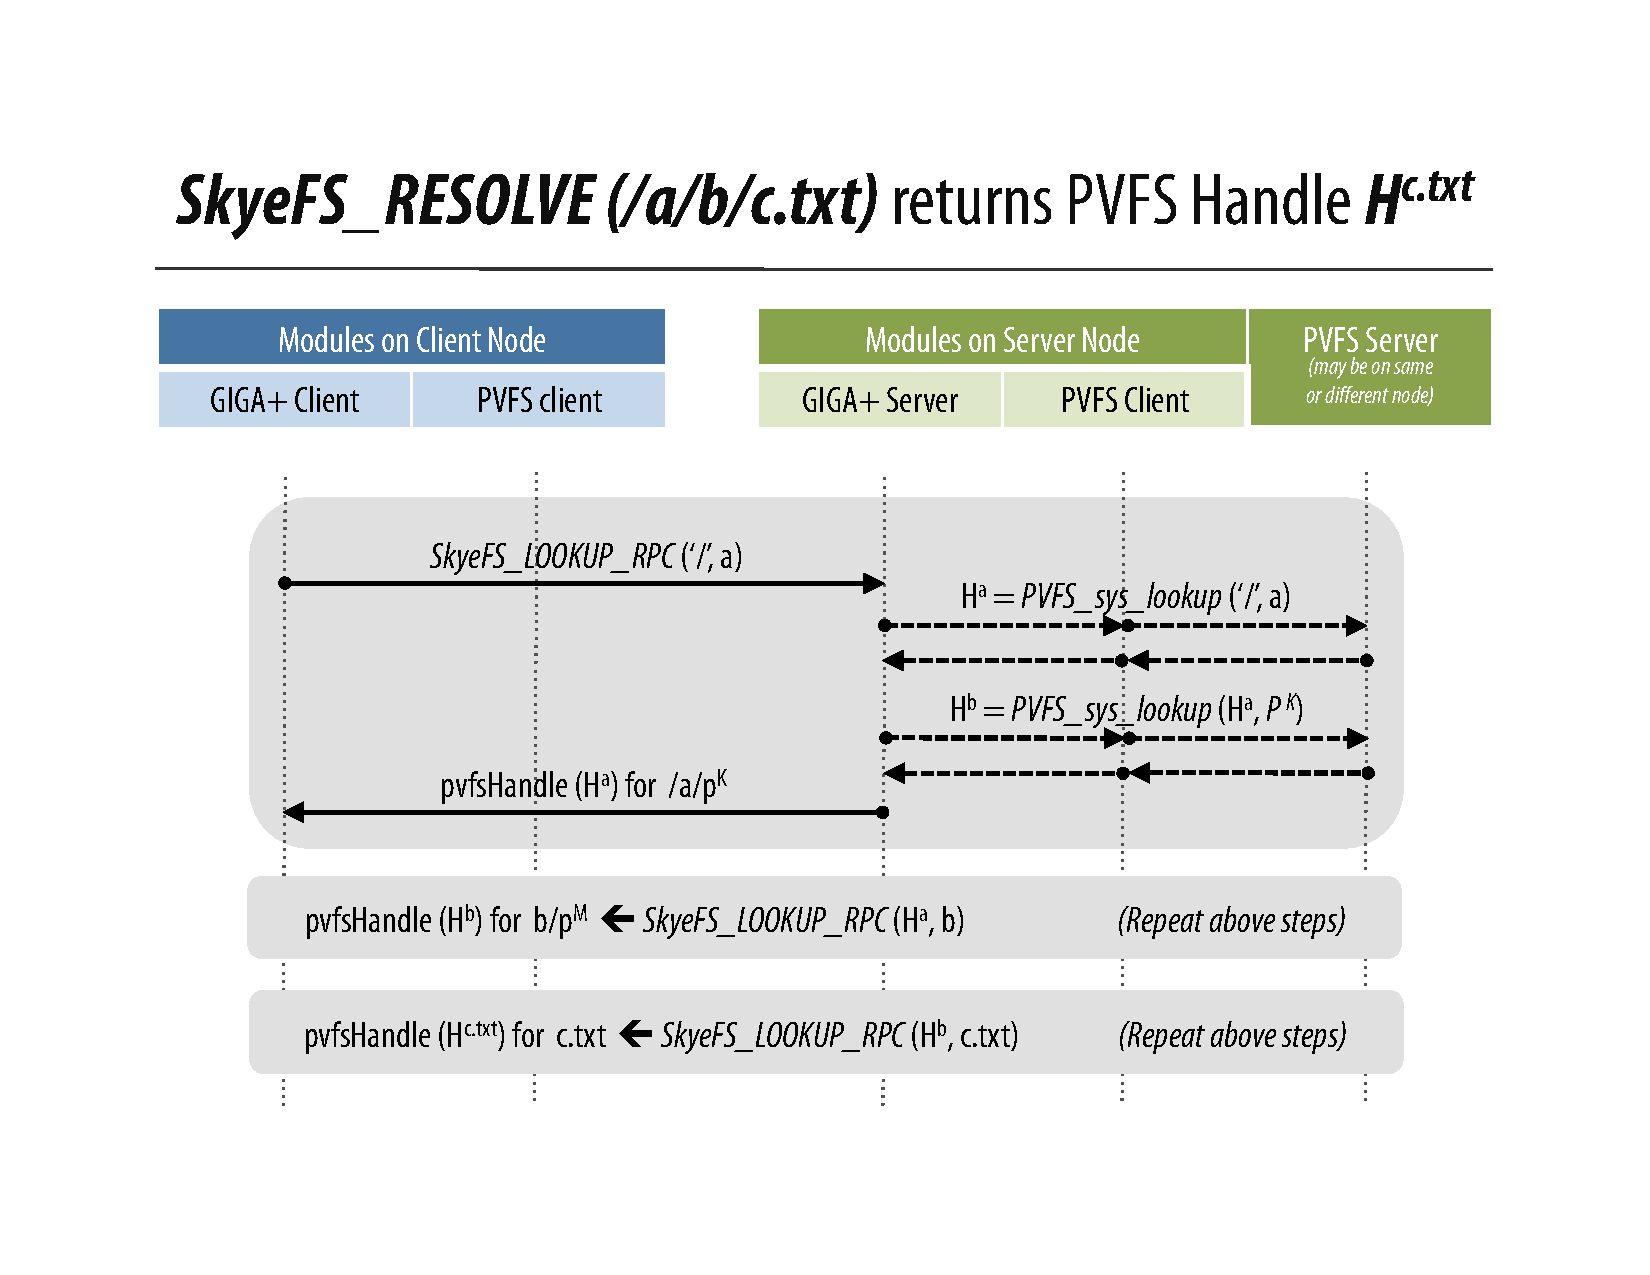
\includegraphics[width=3in]{figure-resolve}
\end{center}
\caption{SkyeFS Name Resolution}
\end{figure}
The FUSE lowlevel API uses a \code{lookup(inode, name)} callback to perform
path resolution.  We use the PVFS handle for an object as the FUSE inode to
avoid keeping a lookup table on the client.  PVFS provides a
\code{PVFS\_\-sys\_\-ref\_\-lookup(handle, name)} which is analogous to the
FUSE \code{lookup} function.  Our \code{skye\_server} wraps this PVFS function
to both resolve the Giga+ partition and the object itself and exposes an
\code{lookup} RPC to accomplish this.  When the \code{skye\_client} receives a
\code{lookup} callback, it consults its cached bitmap (if any) and then
makes an RPC call to the responsible \code{skye\_server}, retrying in the
event that an EAGAIN is returned.  By resolving both the partition and
requested object in the server, we avoid race conditions due to concurrent
splits.  \footnote{For example, issuing the RPC \code{lookup(NULL, ``foo'')}
would return the PVFS handle of ``/p00004/foo'' if ``foo'' was stored in the
fifth partition of the filesystem root.  If we let that handle be $h$, then
\code{lookup($h$, ``bar'')} would return the PVFS handle of
``/p00004/foo/p00002/bar'' if ``bar'' is in the third partition of ``foo''.
In this manor, any logical path can be resolved to its PVFS handle in a manor
opaque to the caller.}

As PVFS metadata handles do not change when their objects are moved between
directories, the handle returned by \code{lookup} is guaranteed to continue to
be a valid reference to the object for the duration of the object's existence.
This is true even if the partition holding an object splits or the logical
directory is moved elsewhere in the directory tree.  As a result, we can
safely return a PVFS handle to FUSE in the form of an inode umber.

\subsection{Metadata Persistence}
All of the metadata required by Giga+ is persisted directly in PVFS.  Whenever
possible, we prefer to rederive metadata from PVFs instead of storing new
Giga+ data.  While this may come at a performance cost, it makes the system
simple to implement and highly resilient to failures by preventing
opportunities for inconsistencies.

The only filesystem-wide metadata is the server list.  Each SkyeFS client and
server queries this information from PVFS directly.  This allows the system
administrator to change server host names or add new servers by modifying only
the PVFS configuration.

The most important piece of per-directory metadata is the Giga+ bitmap.  This
consists of bits indicating the presence (or absence) of each possible
partition, the server number of the zeroth server and  the number of servers
at the time of creation.  To determine the partitions present, we issue a
\code{readdir()} against the directory and parse the resulting directory names
to determine the partition.  Future versions of SkyeFS will use a
distinguishing name for currently splitting partitions to avoid prematurely
adding these to the bitmap and to enable resuming splitting after a failure.
The zeroth server is always the server responsible for the logical directory.
To support server additions, the number of servers at creation can be stored
as an extended attribute on the directory.

\subsection{Client Bootstrap}
To avoid creating additional load on PVFS, the \code{skye\_client} only loads
a subset of the metadata from PVFS.  The first time a directory is accessed,
it is assumed that there is only one partition.  The code can correctly set
the identity of the zeroth server as this can be derived from PVFS handle for
the directory without incurring additional PVFS operations.  If the client
issues a RPC to the \code{skye\_server} for the directory which results in an
EAGAIN error, it takes the bitwise OR of the current bitmap and the server
provided bitmap.  This allows the client bitmap to be filled-in by the server
on demand without incurring additional PVFS operations.

Populating the initial mapping in this way causes the \code{lookup()} code to
always start with the zeroth server in the cache-cold state.  While this
ensures that some progress towards finding the correct server is always made,
it has the potential to cause unbalanced load on servers which act as the
A future optimization might include having the \code{skye\_server} provide a
bootstrap bitmap to clients when returning a \code{lookup()} result for a
directory that is already cached on the server.

\section{Filesystem Operations}
\subsection{Splitting and file creation}
\begin{figure}
\begin{center}
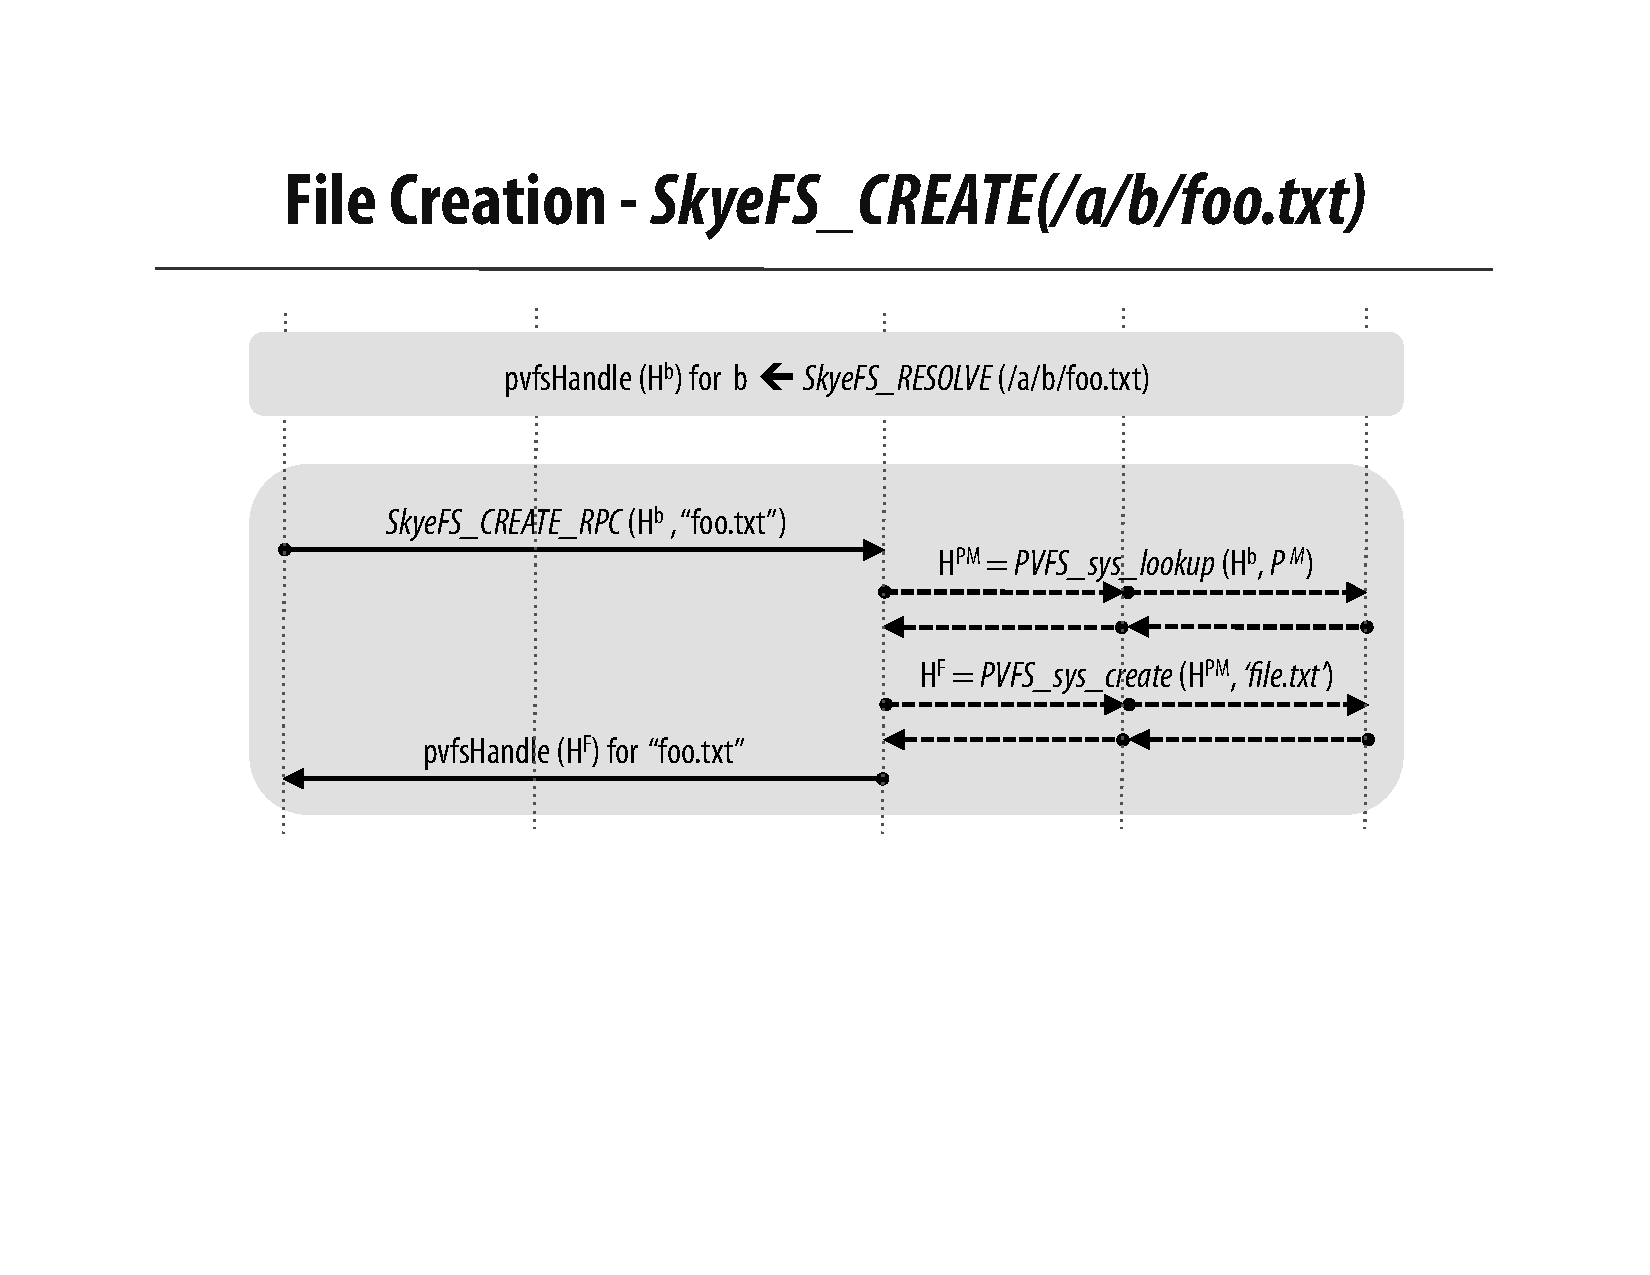
\includegraphics[width=3in]{figure-create}
\end{center}
\caption{SkyeFS Create Procedure}
\end{figure}
The \code{skye\_client} provides a \code{create()} RPC for the
\code{skye\_\-client} to create files in a given directory.  As with all
\code{skye\_server} RPCs, only the server responsible for a partition will
service create requests for that partition.  Each server manages splits for
its partitions and coordinates operations that happen concurrently with a
split.

Splits are triggered in Giga+ when the partition size exceeds a threshold.
The current splitting status is maintained by the \code{splitting\_\-index}
field of the \code{skye\_directory} structure.  When no split is happening,
this field has the value -1; other times it has the number of the currently
splitting partition.  Only one partition per directory may be splitting at one
time under this scheme, however this is a desirable property for performance
reasons.

The \code{skye\_directory} structure contains a read-write lock which is used
to synchronize changes in the splitting state.  Operations that act on the
directory, such as \code{lookup} and \code{create}, take a read lock for their
duration.  When a partition is to be split, the write lock is taken, the
\code{splitting\_index} updated, and then the write lock is dropped.
Similarly, when splitting is complete, the write lock is taken while updating
the \code{splitting\_index}.  This scheme ensures that each operation acting
on a directory has a consistent view of the splitting state of a directory
throughout the operation.  Without this synchronization, a complete bitmap
comparison would be required to determine if a split had interfered with a
concurrent operation making retry and recovery difficult.  The read-write lock
is initialized with the
\code{PTHREAD\_RWLOCK\_PREFER\_WRITER\_NONRECURSIVE\_NP} option to prevent
starving writers.

With a one percent probability, we evaluate the partition of a new object at
the end of each \code{create} operation to see if the partition needs to be
split.  This chick is implemented using the PVFS \code{getattr} operation
which will return the number of directory entries in a directory.  If the
directory size is greater than the split threshold, the partition is added to
a queue of partitions to split and the \code{create} call returns.

Each \code{skye\_\-server} has a dedicated thread for splitting partitions.
This thread waits on a condition variable associated with the split queue.
When a partition is added to the queue, the adding thread signals on the
condition variable to wake up the splitter thread.  Upon waking, the splitter
thread will iterate through the queue, confirming that the partitions are
still over threshold and splitting them if needed.

To split a partition, the splitter thread performs repeated \code{readdir}
operations on the partition to determine the set of candidate entries.  For
each entry, it hashes the name to determine if the object is to be moved to
the new partition and, if so, moves the entry using the PVFS \code{rename}
operation.  This process continues until a complete \code{readdir} of the
directory finds no new entries to move.  In practice, this usually happens on
the third pass.  When the split is complete, a \code{bucket\_\-add} RPC is
sent to the server responsible for the new partition.  This RPC will cause the
new server to add the partition to its bitmap and assume responsibility for
the partition.

While a split is occurring, any thread that accesses the directory will notice
that \code{splitting\_\-index} is not set to -1 allowing the operation to
modify its behavior to operate correctly despite the split.  In the case of
object creation, objects are created in the child partition if that is where
they would be migrated.  In the case of \code{lookup}, both the child and
parent partitions are checked for the object.

We use a separate splitting thread to allow splittings to take place
asynchronously with respect to the \code{create} operations that caused them.
Our locking semantics allow filesystem operations to continue on a partition
during its split.  These features can result in significantly improved
performance over implementations that must block during a split.

\subsection{Directory Creation}
In most respects, \code{mkdir} is implemented identically to \code{create}.
When the \code{skye\_server} creates a directory it also creates that
directory's first partition.  No additional work is done at creation time to
setup Giga+ metadata as the server which creates the directory is usually not
the zeroth server for the new directory.  The first time the new directory is
accessed, the zeroth server will load the Giga+ metadata as if it was simply
an old, but empty, directory.  In the event that a server fails between
creating a directory and its zeroth partition, the directory will be in an
inconsistent state.  However, this can be easily repaired by the server when
such a directory is first accessed.

\subsection{Object Removal}
Removing a file is a relatively simple operation, we simply issue a PVFS
remove for the file.  Currently, we do not remove empty partitions or
coalesce partitions which shrink to below the split threshold.

However, \code{rmdir} presents a challenge because the directory removal must
be coordinated between all servers which are responsible for a partition of
the directory.  Additionally, we must ensure that the remove operation on a
directory will fail if there exist any files in the directory.

To coordinate removal of a directory, we implement a server to server RPC call
called \code{bucket\_\-remove}.  The client attempting to remove a directory
will send a \code{remove} RPC to the server holding the directory entry for
the directory.  The server will then issue a \code{bucket\_\-remove} RPC for
each bucket in descending order (i.e. the highest numbered bucket first).  

When a server receives this call it will attempt to remove the specified
partition by issuing a PVFS \code{remove} for the partition.  If the operation
succeeds then the partition will be removed from the owner's bitmap and the
owner will return a positive response to the caller.  The caller will also
remove the partition from its bitmap and then issue the next
\code{bucket\_\-remove}.

If the PVFS \code{remove} fails (for any reason other than \code{ENOENT}) the
partition will remain in the bitmap and a negative response will be returned
to the server.  The coordinating server will then halt the operation and
return the error to the client.  In this case care must be taken to ensure
that the system is left in a consistent state.  By removing the partitions in
descending order we ensure that we always remove the child of a split before
its parent.  Therefore, each intermediate bitmap (produced between
\code{bucket\_\-remove()} calls) is a valid bitmap in itself.

However, for a client to behave correctly after an aborted \code{rmdir}
operation, we need a mechanism to remove the deleted partitions from the
client bitmap.  As the standard merge operation performed by the client does a
logical OR of the old and new bitmaps it is unable to handle a removal.
Instead, we rely on a fail safe, ``something is wrong'' mechanism.  If a
client receives an \code{EAGAIN} from a server but merging the returned bitmap
does not add any new partitions, the client will assume that something was
removed and simply replace its bitmap with the server provided
one bitmap.  This behavior is not currently implemented in SkyeFS, however
when complete it will also allow for removal or coalescing of partitions as a
directory shrinks.

\subsection{Rename}
The \code{rename} operation is also challenging because it must operate on two
distinct objects that may not be located on the same server.  To solve this we
use an optimistic retry strategy.  The \code{skye\_\-server} implements a
\code{partition} RPC that is similar to \code{lookup} but instead of returning
the handle of the requested object it returns the handle of the encompassing
partition.  The client uses \code{partition} to determine the handle of the
source directory.  This handle (and the source and destination file names)
are passed to the destination partition's \code{skye\_\-server}.  The
\code{skye\_\-server} will attempt to move the file using the provided source
handle and name into the correct destination partition.  

In the event that a split has happened between the \code{partition} call and
the \code{rename} call which caused the source partition to change, the
\code{rename} will return \code{ENOENT}.  The client will the retry the
\code{partition} to see if the partition's handle has changed.  If so, the
rename is retried with the new handle.

This technique eliminates the need for any locks to be held across multiple RPC
calls but is vulnerable to starvation in the event of high rates of splitting.
We believe this this risk of starvation is unlikely to occur in practice due to
the speed at which a split can progress.

\subsection{Directory Listing}
\begin{figure}
\begin{center}
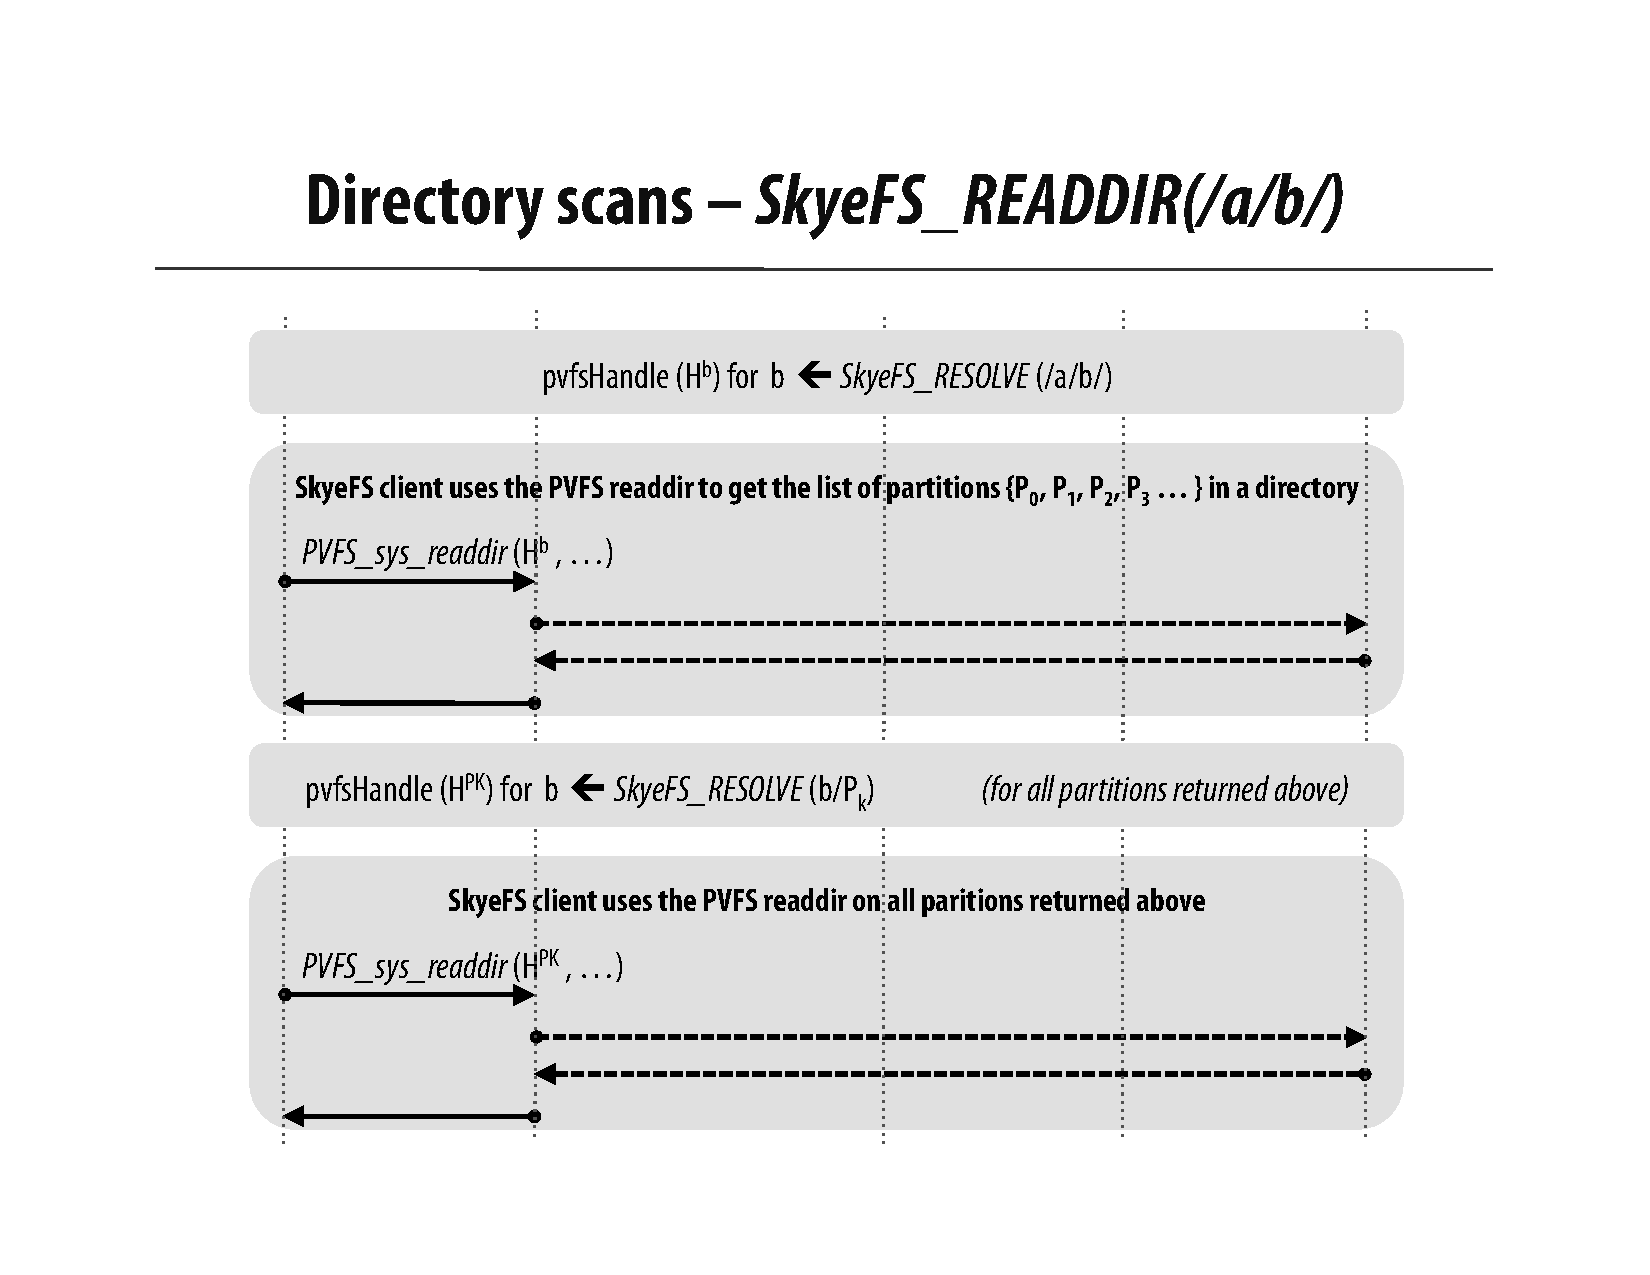
\includegraphics[width=3in]{figure-readdir}
\end{center}
\caption{SkyeFS readdir()}
\end{figure}
To simplify the \code{readdir} and ensure correct semantics, the
\code{skye\_client} implements the actual directory reading during the FUSE
\code{opendir} callback.  The contents of a directory are loaded into an array
from which each subsequent \code{readdir} command is serviced.

Because each Giga+ partition is implemented as a distinct PVFS directory, it
would be very difficult to implement a fully consistent readdir.  Instead, we
make a best effort and avoid costly synchronization.  When the
\code{skye\_client} receives an \code{opendir} call it first issues a PVFS
\code{readdir} on the logical directory itself to get a list of partitions
(both complete and splitting).  The client then iterates through each of these
partitions and issues a PVFS \code{readir} for each partition concatenating
the results.  

While this technique is prove to returning inconsistant results in the case of
concurrent modifications, it places a minimum load on the PVFS servers.
However, it is important to note that this is only an issue for directories
larger than the split threshold and most directories will fall well below this
threshold.  In the future, \code{skye\_client} could aggressively fetch
directory entries from multiple PVFS servers in parallel to complete the
readdir more quickly.

\subsection{Other Operations}
\begin{figure}
\begin{center}
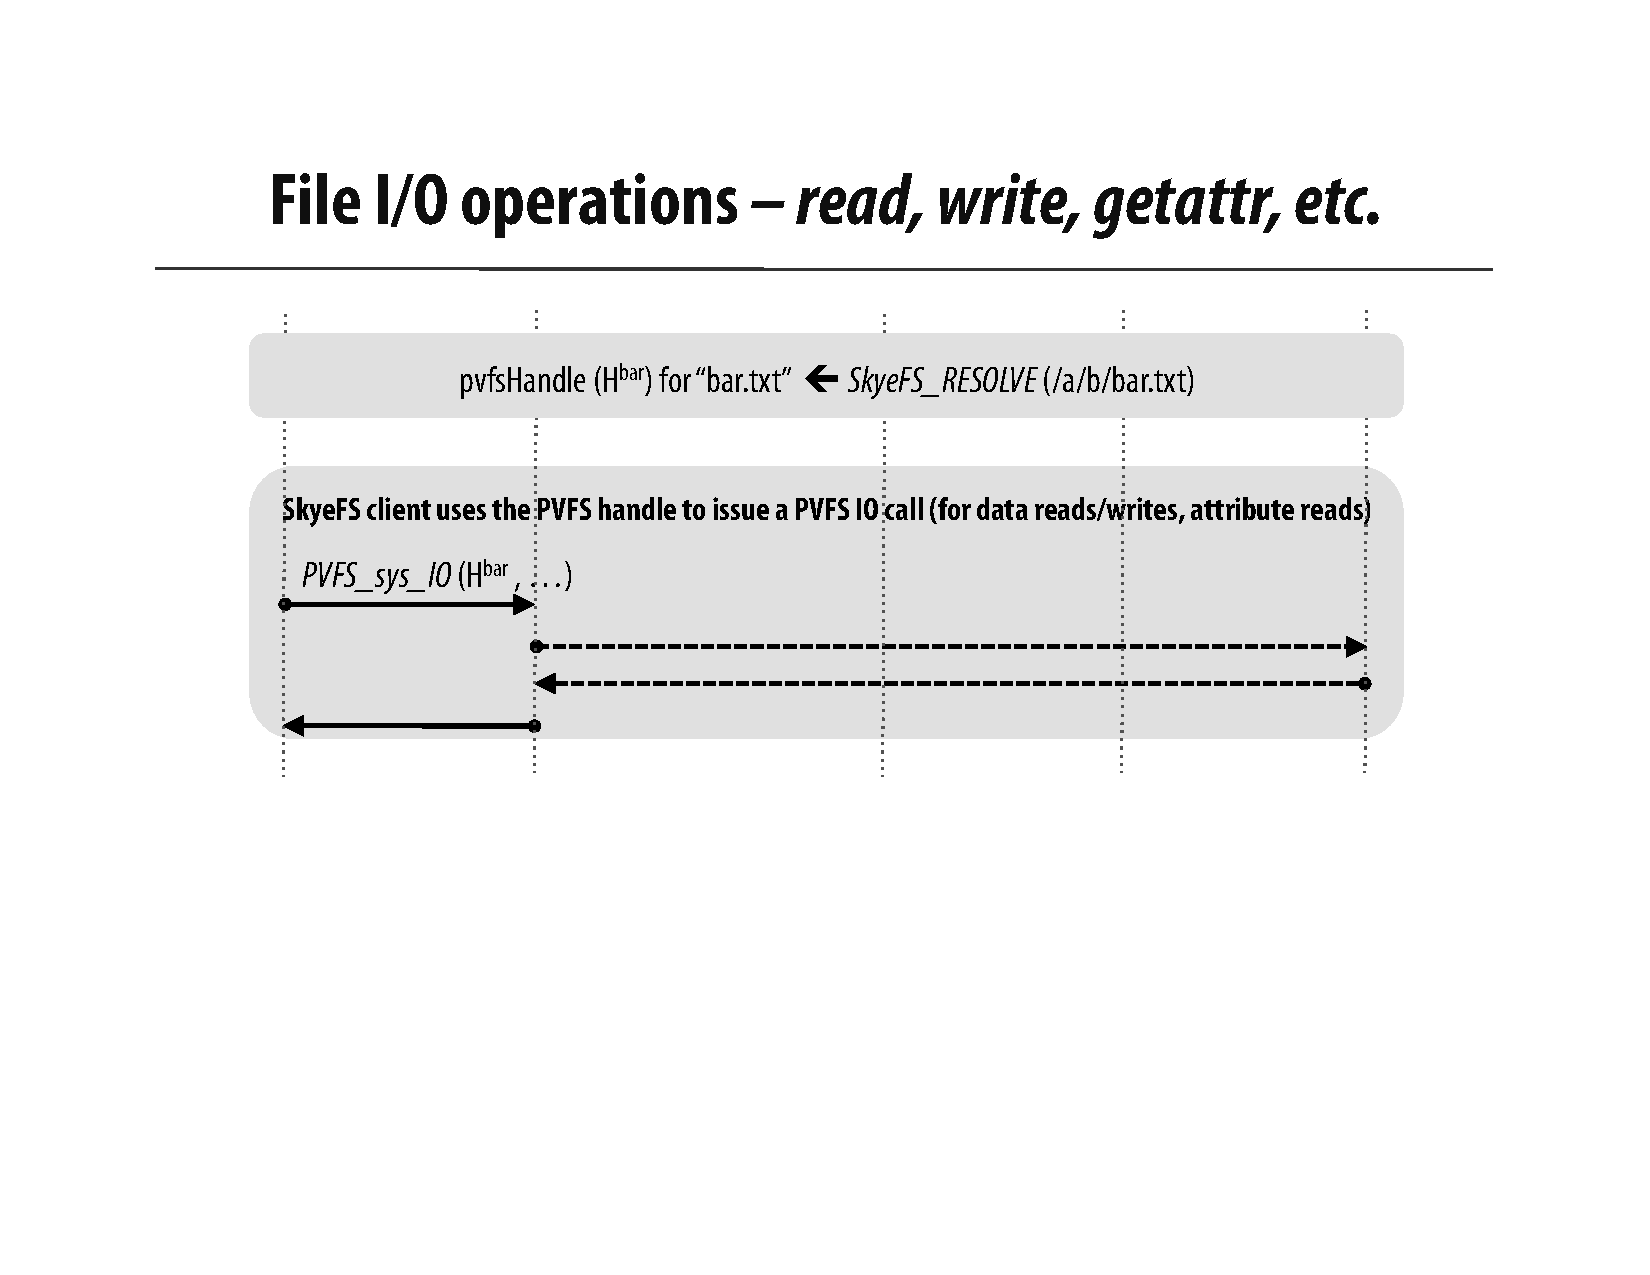
\includegraphics[width=3in]{figure-other}
\end{center}
\caption{SkyeFS IO Operations}
\end{figure}
All other operations are relatively straightforward modifications of their
pvfs2\-fuse counterparts with the PVFS \code{lookup} operation replaced by our
RPC.  This includes both data operations such as \code{read} and \code{write}
as well as metadata operations like \code{stat} and \code{chmod}.  Because we
resolve all objects to PVFS handles inside their Giga+ partitions, these
operations can proceed on the client without concern for future splitting.

\section{Other Considerations}
\subsection{Multi-step Lookup}
In the current system, a \code{lookup} call can only descend one step in a path
traversal.  Future work could extend the operation to provide the entire path
to the \code{skye\_\-server} and allow the server to descend as many
directories in the path as it owns.  This would be of limited value in the
current system where the servers for a parent and child directory are chosen
independently.  At the cost of load balancing, parent and child directories
could be placed often on the same server to allow this mechanism to speed
directory lookups.  One example scheme to achieve this would be to place all
new directories on the same server as their parent.  When a directory splits
the first time the zeroth server would be moved to a new server chosen at
random.  This would have the effect of keeping strings of small (and likely
low-traffic) directories on the same server while still ensuring that large
directories are load-balanced.

\subsection{Server Addition}
PVFS includes very limited support for server addition.  While new servers can
be added to the configuration file for a filesystem and brought online they must
take a previously unoccupied part of the handle space and there exists no
mechanism for automatically migrating either data or metadata to the new server.
The current SkyeFS implementation includes no specific provisions for addition
of servers, however future work could use SkyeFS to support the migration of
some data to new PVFS MDS.  In particular, by splitting overfull but already
load-balanced directories to these new servers some load can be moved to the
servers in already existing directories.  Because SkyeFS stores the number of
servers existing at the time of creation in each directory as an extended
attribute of that directory,\footnote{This is currently unimplemented.} no
specific mechanism is needed to add a new server other than adding the server
to the PVFS cluster and restarting all \code{skye\_\-server} processes.  However,
this mechanism is untested.

\subsection{Fault Tolerance}
PVFS is not a redundant file system and so it has very limited support for fault
tolerant or highly available configurations.  As a result, we do not make any
attempts to provide redundant services or fall over support in the case of
failures.  We assume that \code{skye\_\-server} processes and the PVFS servers fail
together and that any failure will render the system unusable until resolved by
restarting the system.

However, we do make every effort to leave the system in a consistant state at
all times should any component fail.  Any skye process can fail at any time
and the resulting state will be repaired transparently upon restart.  This is
primarily due to the lack of additional SkyeFS metadata that is required on
top of the PVFS file system.  By carefully controlling the sequence of actions
we take on the PVFS file system we are able to ensure that any state of PVFS
is recognizable as either complete or the result of an unfinished action which
can then be resumed or aborted.

\section{Correctness}
To ensure correctness of the system, we tested against a modified version of
FreeBSD's fstest suite.\cite{fstest} Our version was limited to the tests for
\code{chflags}, \code{chmod}, \code{chown}, \code{mkdir}, \code{open},
\code{readdir}, \code{rename}, \code{rmdir} and \code{unlink}.  We removed
tests that required hard links, which SkyeFS does not support.

\section{Performance Analysis}

\subsection{Method}
Tests were performed on the Marmot cluster consisting of 128 nodes with two
single core Opteron CPUs, 16GiB of RAM, one SATA disk and Gigabit Ethernet.
PVFS was configured with default settings.  In production configurations, we
expect that PVFS would be run on fast disk arrays.  To prevent the single 7200
RPM disks available from artificially limiting throughput, we ran all
experiments with PVFS configured to use a tmpfs for storage.  In each
experiment, both the clients and servers were located on the same set of
machines

\subsection{File Creation}
\begin{figure}
\begin{center}
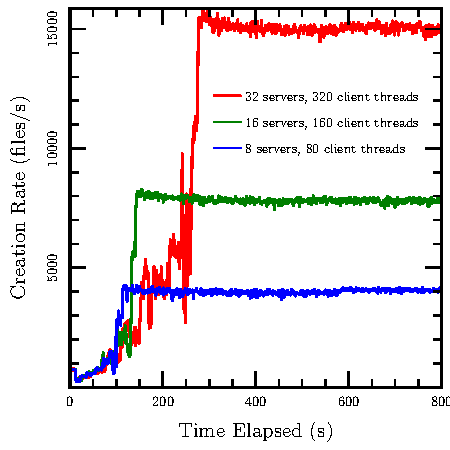
\includegraphics[width=3in]{graph-create}
\end{center}
\caption{SkyeFS Empty File Creation Throughput}
\end{figure}

To test directory insert rates we started with an empty filesystem and created
a single directory.  For each server, we started 10 clients simultaneously
which all attempted to insert uniquely named files into the directory.  We
recorded the overall rate of inserts in the entire system.

For 32 servers, the system reached a peak throughput of over 15k creates per second
after 4 minutes and 30 seconds.  For 16 servers, peak throughput was 8k
creates per second after 2 minutes and 25 seconds.  And for 8 servers, peak
throughput was 4k creates per seconds after 1 minutes and 55 seconds.

This experiment provides the expected linear scaling of throughput after the
system has become load balanced.  We believe the increased time required to
get to a load-balanced state for the 32 server experiment is due to higher
resource contention during the first few splits.  Future work might look at
ways to quicken these first few splits in the event of very high load to
prevent this problem.

We note that the use of FUSE turns each \code{mknod} into a pair of
\code{lookup} and \code{mknod} requests.  The use of the SkyeFS operations
directly, e.g. as part of a shared library, might be able to drastically
improve this performance by avoiding the superfluous \code{lookup}.

\subsection{Readdir}
\begin{figure}
\begin{center}
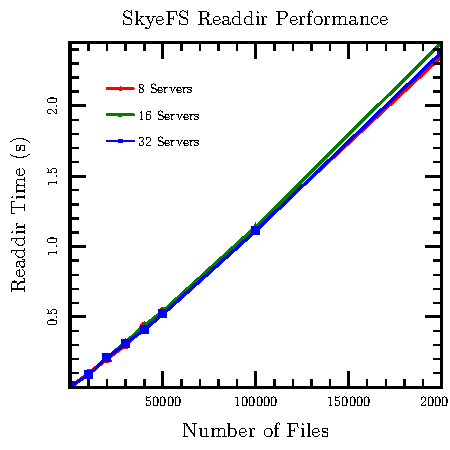
\includegraphics[width=3in]{graph-readdir}
\end{center}
\caption{SkyeFS Readdir Performance}
\end{figure}
One of the desirable properties of the Giga+ algorithm is that it keeps the
overhead for a \code{readdir} small in the case of small directories.  To test
this, we created directories of various sizes and measured the time it took a
single client to read all the entries in the directory.  We repeated this
experiment with 8, 16, and 32 servers.

The client was able to complete a \code{readdir} for a directory with 1000
entries in 0.1 seconds.  As expected, this increased slightly worse than
linearly as the number of entries and partitions increased.  In the case of
200k entries, a \code{readdir} took approximately 2.4 seconds.  No significant
difference in performance was noted between the different server
configurations.

Further work might improve upon this performance by issuing the \code{readdir}
for each partition in parallel.

\subsection{FUSE Low Level API}
Our initial prototype system used the standard FUSE ``high level'' API.  This
API provides a full pathname for every operation.  As a result, each
\code{mknod} call in our file creation experiment required resolving the PVFS
path from the root of the filesystem.  This created an excessive amount of
traffic on the server responsible for the filesystem root and bottlenecked the
system.  We were able to resolve this problem by switching to the lowlevel API
and running our benchmark utility from within the directory in which the files
are to be created.

\subsection{SkyeFS Client and PVFS}
Our initial prototype included a fully multi-threaded client.  However, we
quickly noticed that executing many operations in parallel (for example,
using \code{make -j8} would result in long stalls while executing PVFS calls.
To work around this problem, we currently run the client in the single
threaded FUSE mode.

The FUSE lowlevel API allows the filesystem to return from the callback
without returning a result to FUSE.  After consulting with the PVFS
developers, it has been suggested that using this functionality along with the
asynchronous PVFS operations might allow concurrent operation without
experiencing these stalls.  This was not attempted for this project because of
the large engineering effort required to convert each operation to persist its
state across asynchronous PVFS calls.

\subsection{SkyeFS Server and PVFS}
The \code{skye\_server} is based on the initial Giga+ prototype and uses a
single thread to handle each incoming RPC connection.  As a result, it is easy
for upwards of 100 client operations to be in flight concurrently.  The PVFS
system interface keeps an array of state machines for all outstanding
operations in the address space.  All threads which have an in-flight
operation attempt to take a lock on this array and the thread which acquires
the lock drives progress on all state machines in the array.

The first problem that results from this design is that the array is of
limited size.  Currently, the PVFS code statically defines the array of state
machines to be of length 256.  If an incoming operation would overflow this
array, an assertion is tripped.  To avoid tripping this insertion we
implemented flow control in the form of a semaphore.  When the server starts
the semaphore is initialized to a small value.  When a thread receives an RPC
request, it downs the semaphore before issuing any PVFS requests.  When the
thread completes its work, it will up the semaphore.  In this way, we prevent
more than the semaphore's initial value threads from issuing PVFS requests
concurrently.  In practice, we found that we needed to set this initial value
as low as 32 to avoid tripping the assert.

The other problem with this design is that it does not guarantee fairness to
the requests on the array.  This means that while a request may have
completed, the requesting thread may not notice this for a very long time.
This introduces significant jitter into client response times and slows the
entire system's throughput as a client is unnecessarily blocked on a server
response.  To solve this problem, we further restrict the number of concurrent
operations in flight by initializing our flow control semaphore to 12.
Our testing indicated that this value is optimal in the 32 server case.

\subsection{Split Performance}
\label{section:splitperf}
During a split the split thread must issue \code{readdir} calls to the
partition which is being split.  While this is happening, additional creates
may be issued against that partition.  We found that without external
synchronization, this pattern of requests results in very poor PVFS
performance.

We wrote a test program to isolate this particular workload.  The program
connects to a provided PVFS server using the system interface.  It then spawns
10 threads which all create files in that directory until 5000 files are
created.  It also spawns another thread that will list out the contents of
that directory repeatedly, reporting the time taken each time.  The program
supports three synchronization models for the threads to test different levels
of interleaving of requests.

In the unsynchronized model all threads are allowed to run without any
synchronization.  On our test system, this required 42 seconds and the
directory listings took between 2 and 12 seconds to complete with a median of
7 seconds.

In our create-synchronized model, each of the 10 threads that issue creates
synchronizes on a single mutex such that only one create is every in flight at
a time.  With this model, 41 seconds were required to create the files and the
listings took between 2 and 20 seconds to complete.

In our final, everything synchronized model, all create threads and the
readdir thread synchronized on the same mutex.  With this model, the creates
take 43 seconds to complete and all listings take less than 200ms.

To overcome the PVFS stalls in the unsynchronized and create-synchronized
models, our splitter thread initially drops the write lock after updating the
\code{splitting\_index} but then reacquires the write lock for each set of
\code{readdir + rename} operations.  This allows some degree of concurrency
(outstanding operations can complete between each set of operations) while
still preventing the observed stall.
\section{Related Work}
SkyeFS implements the Giga+ technique for distributing filesystem metadata
presented in \cite{gigaplus}.  As discussed in \cite{gigaplus}, Giga+ builds
on a wide range of previous work on distributed file systems and data
structures.  We adapt the code from the initial Giga+ prototype for use on a
distributed file system (DFS) and show that the scalability results seen by
the initial prototype can be seen when Giga+ is implemented in the context of
a DFS.

SkyeFS also builds on the FUSE module for the Linux kernel and the PVFS client
library to provide filesystem services and consume PVFS services respectively.
The \code{pvfs2-fuse} application distributed with PVFS provided valuable
insight on how to bridge between the FUSE API and the PVFS API.  When
possible, portions of code from this application were used verbatim.

OrangeFS is a native implementation of Giga+ in PVFS.\cite{orange}  OrangeFS
shows similar scaling performance to SkyeFS, however it lacks the ability to
incrementally grow the number of partitions in a directory.

\section{Conclusion}
We successfully implemented Giga+ distributed directories on top of PVFS.  We
demonstrated that the capabilities provided by PVFS are sufficient for a high
performance implementation of distributed directories without requiring
modification to PVFS itself.  This shim technique may be adaptable to
implementation of distributed metadata on other distributed filesystems.
We've shown that Giga+ is capable of achieving near linear speedup once a
directory is at load balance.  We've also demonstrated that Giga+ preserves
the desired responsiveness properties of PVFS in the case of small
directories.  We note that future work is needed to overcome performance
problems in PVFS exposed by the SkyeFS workloads.


\newpage
\small

\section*{Acknowledgements}
We'd like to thank Sam Lang and Phil Carns for their advice and assistance in
working with PVFS.  This material is based upon research supported in part by
the Notional Science Foundation under contract NFS CNS-1042543 (PRObE) and
the Los Alamos National Lab under contract number DE-AC52-06NA25396 (IRHPIT).
We also thank the members and companies of the PDL Consortium (including
Actifio, American Power Conversion, EMC Corporation, Emulex, Facebook,
Fusion-io, Google, Hewlett-Packard Labs, Hitachi, Huawei Technologies Co.,
Intel Corporation, Microsoft Research, NEC Laboratories, NetApp, Inc., Oracle
Corporation, Panasas, Riverbed, Samsung Information Systems America, Seagate
Technology, STEC, Inc., Symantec Corporation, VMware, Inc., Western Digital)
for their interest and support.

\begin{thebibliography}{9}

  \bibitem{gigaplus}
    Patil, S. and Gibson, G. Scale and Concurrency of GIGA+: File System
    Directories with Millions of Files.
    Proceedings of FAST '11: 9th USENIX Conference on File and Storage
    Technologies.
    \url{http://www.pdl.cmu.edu/PDL-FTP/PDSI/CMU-PDL-08-110_abs.shtml}

  \bibitem{pvfs}
    P. H. Carns, R. B. W. B. Ligon III, and R. Thakur. PVFS: A Parallel File
    System For Linux Clusters. Proceedings of the 4th Annual Linux Showcase
    and Conference, 2000.
    \url{http://ftp.mcs.anl.gov/pub/tech_reports/reports/P804.pdf}

  \bibitem{orange}
    S. Yang, W. Ligon, and E. Quarles. Scalable Distributed Directory
    Implementation on Orange File System. 7th IEEE International Workshop on
    Storage Network Architecture and Parallel I/O, 2011.
    \url{http://storageconference.org/2011/Papers/SNAPI/6.Yang.pdf}

  \bibitem{rpc}
    Srinivasan, R. RPC: Remote Procedure Call Protocol Specification Version 2.
    RFC 1831, Aug. 1995.

  \bibitem{fuse}
    FUSE. Filesystem in Userspace. \url{http://fuse.sf.net}

  \bibitem{fstest}
  Pawel Dawidek.  fstest from FreeBSD.  \url{http://people.freebsd.org/~pjd/fstest/}

\end{thebibliography}
\end{document}
